% An example second appendix from the example thesis thesis.tex.
\chapter{EE 518 Test Results}

\section*{E E 518 Lab Tests}

Further testing of the square-law detector was performed by using the radiometer in a real world event.  This test was exercised in conjunction with the Microwave Remote Sensing class (E E 518) under Dr. Brian Hornbuckle.  In 2012 the radiometer was moved to the roof of agronomy and the EE 518 students conducted a number of tests using the N200 software defined radio to collect the data.


{\begin{figure}[h!tb] 
\centering
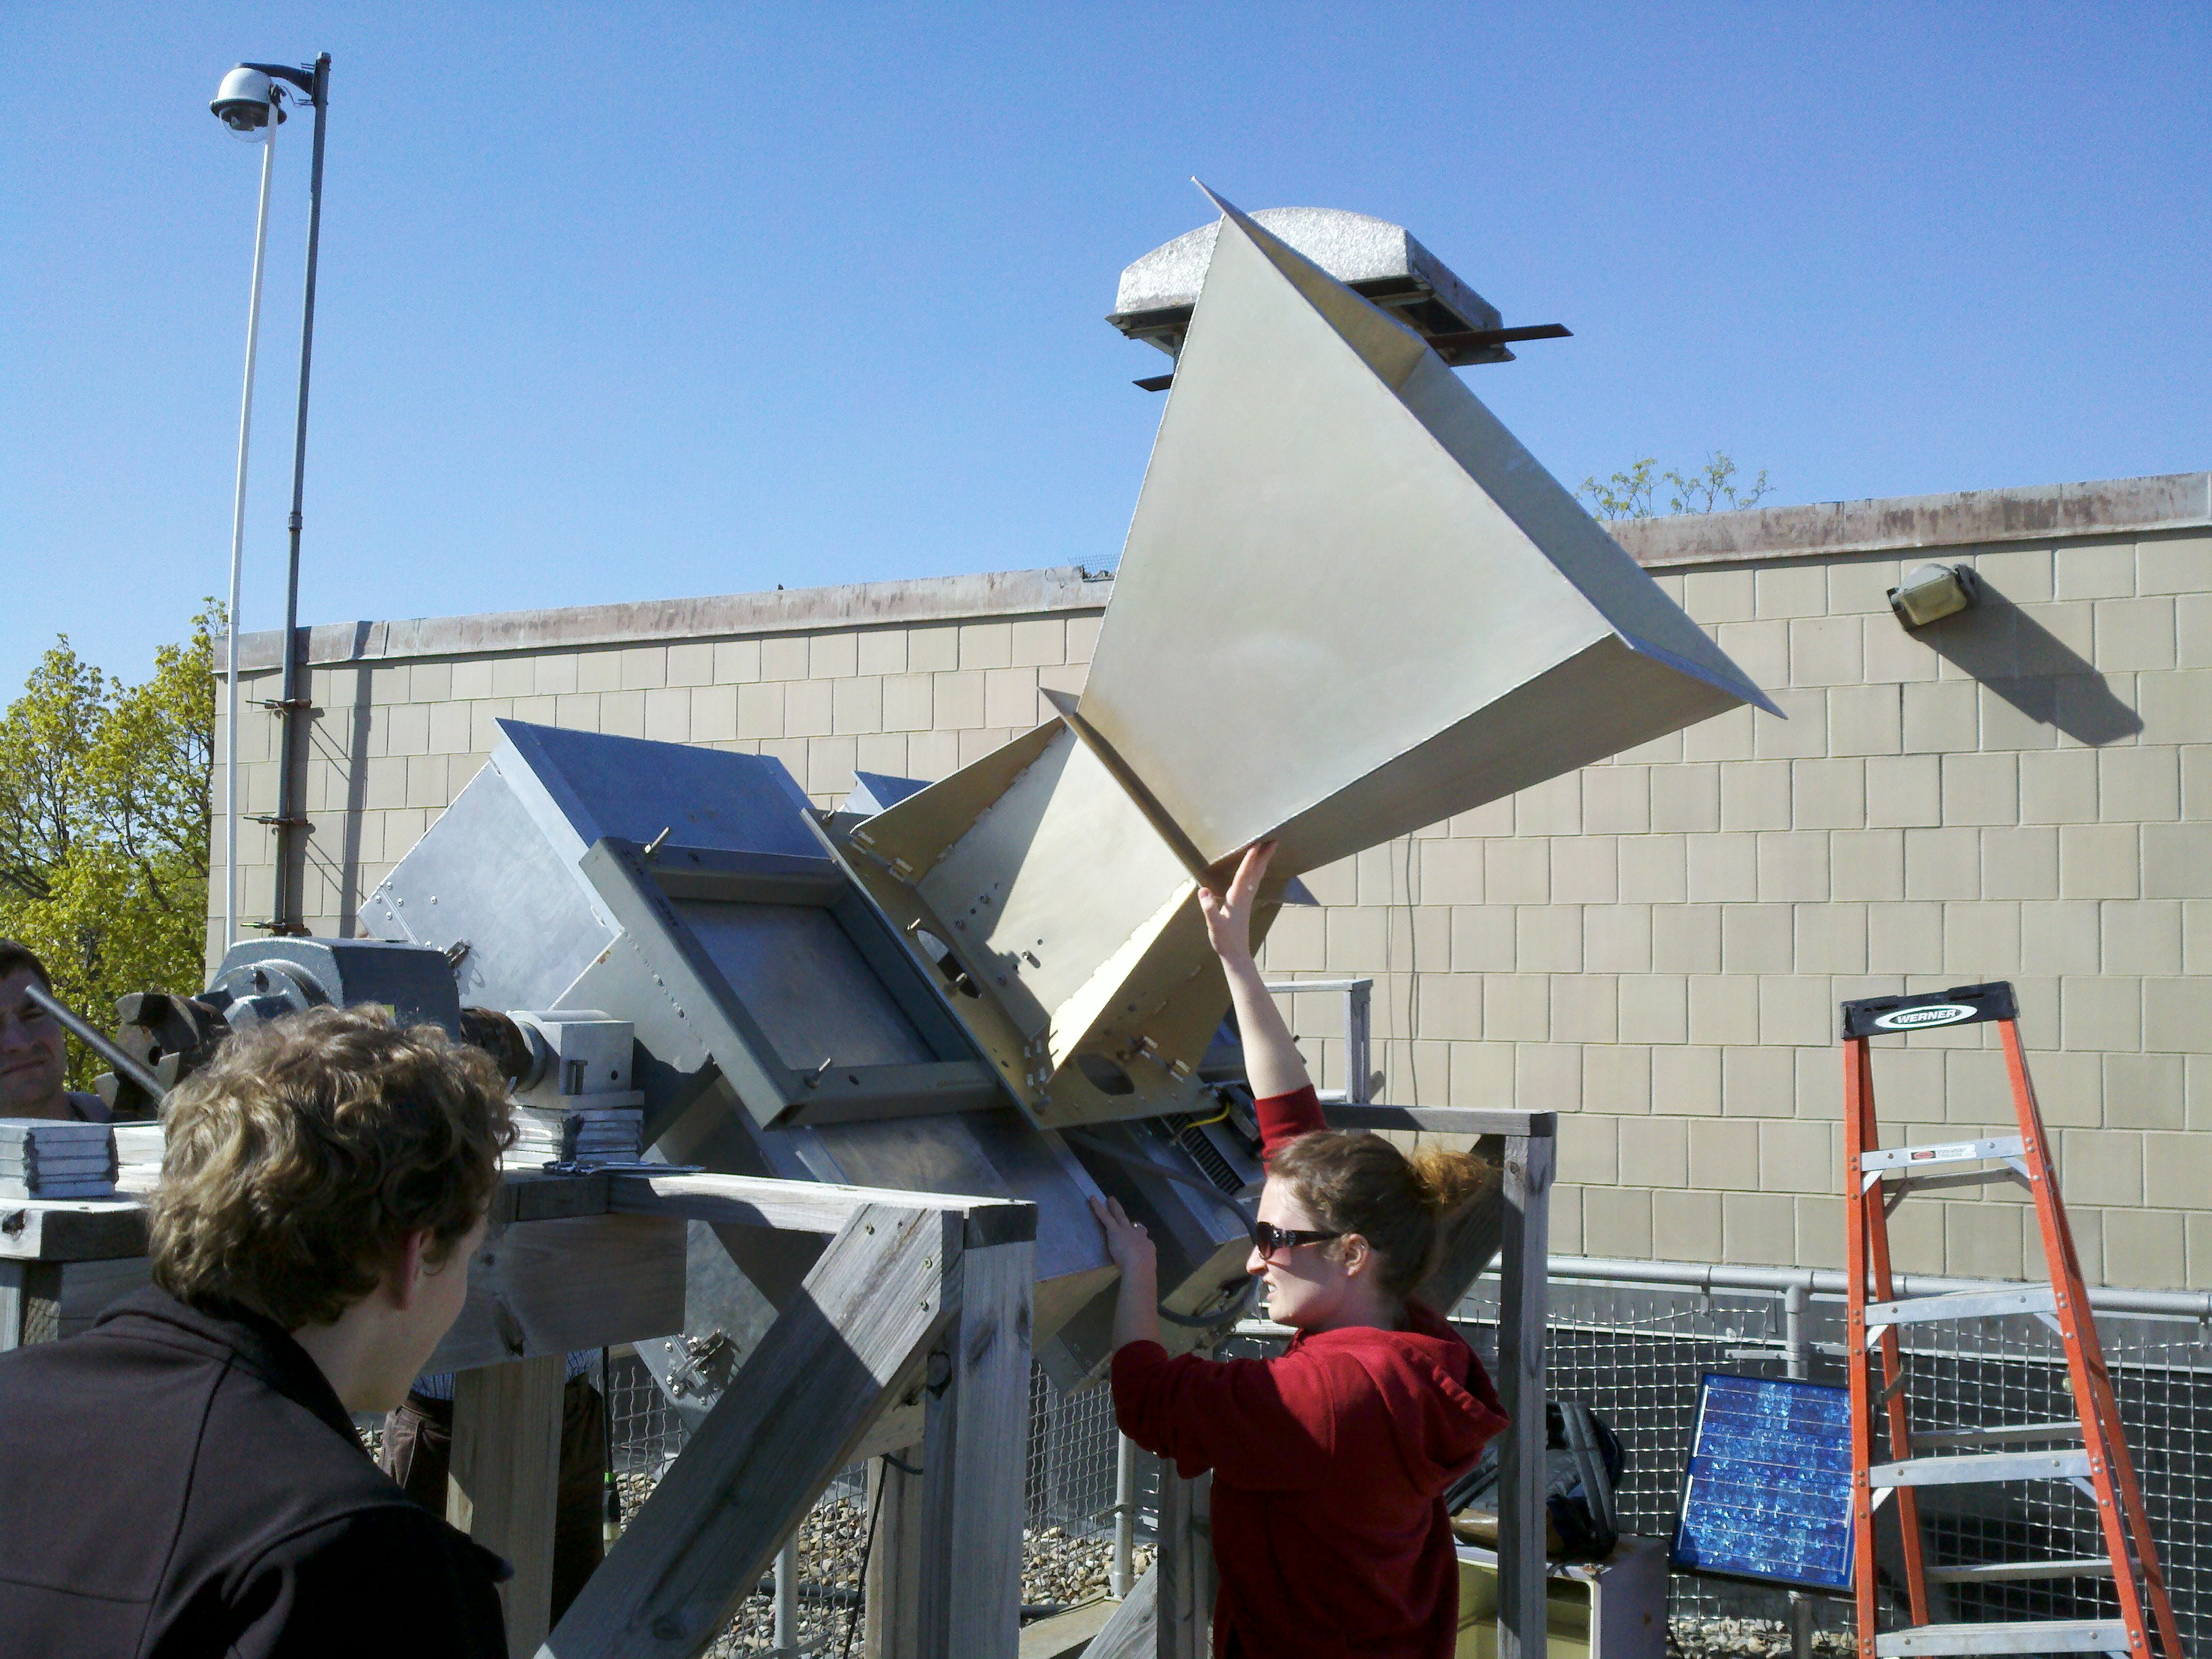
\includegraphics[width=\textwidth]{Images/radiometer_roof.jpg}
\isucaption{Students rotating the radiometer for an experiment on Agronomy Hall}
\label{radiometer_roof}
\end{figure}
}

The E E 518 test however showed that there were additional problems with the radiometer.  While the test showed that the SDR could in fact read data, the data was skewed.  It was later found out that the radiometer was generating an interfering signal that caused the power readings to be elevated.  That was found as a result of having the SDR record the signal and then was analyzed later.  Through this analysis, we found that a strong harmonic was developed and caused a spike in signal being recorded.  Although the exact reason for this has not been found, the problem has been isolated to something in the RF Front End of the ISU radiometer. 

In 2014 the E E 518 class ran another experiment, but this time a different one.  This experiment mimicked the experiments that I ran to calibrate and test the radiometer.  This allowed an outside source to validate the results that I was getting with running the radiometer.  Like my tests, the students submerged a matched load into liquid nitrogen and then in boiling water.  The liquid nitrogen was assumed to be at 77 K and the boiling water was measured to be at 99 C or 372 K.  The students were then given a mystery sample in which they had to determine the temperature of a water sample.  Since the students had to points, they could find the calibration line and determine the temperature.  The experiment was run twice as we expected the radiometer may have drifted between measurements.  